\begin{tikzpicture}
\coordinate (d1) at (0,2,0);
\node (d2) at (0,-1,0) {$\text{C}_6$};
\draw[red] (d1) -- (d2);
\begin{scope}[canvas is xz plane at y=0]
\coordinate (a) at (xyz spherical cs: radius=1, longitude=0);
\coordinate (b) at (xyz spherical cs: radius=1, longitude=60);
\coordinate (c) at (xyz spherical cs: radius=1, longitude=120);
\coordinate (d) at (xyz spherical cs: radius=1, longitude=180);
\coordinate (e) at (xyz spherical cs: radius=1, longitude=240);
\coordinate (f) at (xyz spherical cs: radius=1, longitude=300);
\draw  (a) -- (b) -- (c) -- (d) -- (e) -- (f) -- (a);
\end{scope}
\begin{scope}[canvas is xz plane at y=1.5]
\coordinate (s) at (xyz spherical cs: radius=0);
\end{scope}
\draw (a) -- (s);
\draw (b) -- (s);
\draw (c) -- (s);
\draw (d) -- (s);
\draw (e) -- (s);
\draw (f) -- (s);
\coordinate (t) at (1.5,0,1.5);
\coordinate (u) at (-1.5,0,1.5);
\coordinate (v) at (-1.5,0,-1.5);
\coordinate (w) at (1.5,0,-1.5);
\draw (t) -- (u) -- (v) -- (w) -- (t);
\fill[nearly transparent, blue] (t) -- (u) -- (v) -- (w) -- (t);
\end{tikzpicture}
\begin{tikzpicture}
\coordinate (d1) at (0,2,0);
\node (d2) at(0,-2,0) {$\text{D}_6$};
\draw[red] (d1) -- (d2);
\begin{scope}[canvas is xz plane at y=1]
\coordinate (pa) at (xyz spherical cs: radius=1, longitude=0);
\coordinate (pb) at (xyz spherical cs: radius=1, longitude=60);
\coordinate (pc) at (xyz spherical cs: radius=1, longitude=120);
\coordinate (pd) at (xyz spherical cs: radius=1, longitude=180);
\coordinate (pe) at (xyz spherical cs: radius=1, longitude=240);
\coordinate (pf) at (xyz spherical cs: radius=1, longitude=300);
\draw  (pa) -- (pb) -- (pc) -- (pd) -- (pe) -- (pf) -- (pa);
\end{scope}
\begin{scope}[canvas is xz plane at y=0]
\coordinate (a) at (xyz spherical cs: radius=1, longitude=0);
\coordinate (b) at (xyz spherical cs: radius=1, longitude=60);
\coordinate (c) at (xyz spherical cs: radius=1, longitude=120);
\coordinate (d) at (xyz spherical cs: radius=1, longitude=180);
\coordinate (e) at (xyz spherical cs: radius=1, longitude=240);
\coordinate (f) at (xyz spherical cs: radius=1, longitude=300);
\draw[dashed]  (a) -- (b) -- (c) -- (d) -- (e) -- (f) -- (a);
\end{scope}
\begin{scope}[canvas is xz plane at y=-1]
\coordinate (ma) at (xyz spherical cs: radius=1, longitude=0);
\coordinate (mb) at (xyz spherical cs: radius=1, longitude=60);
\coordinate (mc) at (xyz spherical cs: radius=1, longitude=120);
\coordinate (md) at (xyz spherical cs: radius=1, longitude=180);
\coordinate (me) at (xyz spherical cs: radius=1, longitude=240);
\coordinate (mf) at (xyz spherical cs: radius=1, longitude=300);
\draw  (ma) -- (mb) -- (mc) -- (md) -- (me) -- (mf) -- (ma);
\end{scope}
\draw (pa) -- (ma);
\draw (pb) -- (mb);
\draw (pc) -- (mc);
\draw (pd) -- (md);
\draw (pe) -- (me);
\draw (pf) -- (mf);
\coordinate (t) at (1.5,0,1.5);
\coordinate (u) at (-1.5,0,1.5);
\coordinate (v) at (-1.5,0,-1.5);
\coordinate (w) at (1.5,0,-1.5);
\draw (t) -- (u) -- (v) -- (w) -- (t);
\fill[nearly transparent, blue] (t) -- (u) -- (v) -- (w) -- (t);
\end{tikzpicture}
\begin{tikzpicture}
\coordinate (d1) at (0,2,0);
\node (d2) at (0,-1,0) {$\text{A}_4$};
\draw[red] (d1) -- (d2);
\begin{scope}[canvas is xz plane at y=0]
\coordinate (a) at (xyz spherical cs: radius=1, longitude=0);
\coordinate (b) at (xyz spherical cs: radius=1, longitude=120);
\coordinate (c) at (xyz spherical cs: radius=1, longitude=240);
\draw  (a) -- (b) -- (c) -- (a);
\end{scope}
\begin{scope}[canvas is xz plane at y=1.5]
\coordinate (s) at (xyz spherical cs: radius=0);
\end{scope}
\draw (a) -- (s);
\draw (b) -- (s);
\draw (c) -- (s);
\coordinate (t) at (1.5,0,1.5);
\coordinate (u) at (-1.5,0,1.5);
\coordinate (v) at (-1.5,0,-1.5);
\coordinate (w) at (1.5,0,-1.5);
\draw (t) -- (u) -- (v) -- (w) -- (t);
\fill[nearly transparent, blue] (t) -- (u) -- (v) -- (w) -- (t);
\end{tikzpicture}
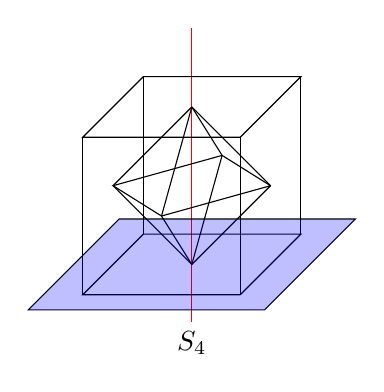
\begin{tikzpicture}
\coordinate (d1) at (0,3,0);
\node (d2) at( 0,-1,0) {$S_4$};
\draw[red] (d1) -- (d2);
\coordinate (os1) at (0,2,0);
\coordinate (os2) at (0,0,0);
\coordinate (oa) at (1,1,0);
\coordinate (ob) at (0,1,-1);
\coordinate (oc) at (-1,1,0);
\coordinate (od) at (0,1,1);
\draw (oa) -- (ob) -- (oc) -- (od) -- (oa);
\draw (oa) -- (os1);
\draw (oa) -- (os2);
\draw (ob) -- (os1);
\draw (ob) -- (os2);
\draw (oc) -- (os1);
\draw (oc) -- (os2);
\draw (od) -- (os1);
\draw (od) -- (os2);
\coordinate (pa) at (1,2,1);
\coordinate (pb) at (1,2,-1);
\coordinate (pc) at (-1,2,1);
\coordinate (pd) at (-1,2,-1);
\draw (pa) -- (pb) -- (pd) -- (pc) -- (pa);
\coordinate (a) at (1,0,1);
\coordinate (b) at (1,0,-1);
\coordinate (c) at (-1,0,1);
\coordinate (d) at (-1,0,-1);
\draw (a) -- (b) -- (d) -- (c) -- (a);
\draw (a) -- (pa);
\draw (b) -- (pb);
\draw (c) -- (pc);
\draw (d) -- (pd);
\coordinate (t) at (1.5,0,1.5);
\coordinate (u) at (-1.5,0,1.5);
\coordinate (v) at (-1.5,0,-1.5);
\coordinate (w) at (1.5,0,-1.5);
\draw (t) -- (u) -- (v) -- (w) -- (t);
\fill[nearly transparent, blue] (t) -- (u) -- (v) -- (w) -- (t);
\end{tikzpicture}
\begin{tikzpicture}
\coordinate (d1) at (0,2,0);
\node (d2) at(0,-2,0) {$A_5$};
\draw[red] (d1) -- (d2);
\begin{scope}[canvas is xz plane at y=0.5]
\coordinate (pa) at (xyz spherical cs: radius=1, longitude=0);
\coordinate (pb) at (xyz spherical cs: radius=1, longitude=360/5);
\coordinate (pc) at (xyz spherical cs: radius=1, longitude=360/5*2);
\coordinate (pd) at (xyz spherical cs: radius=1, longitude=360/5*3);
\coordinate (pe) at (xyz spherical cs: radius=1, longitude=360/5*4);
\draw  (pa) -- (pb) -- (pc) -- (pd) -- (pe) -- (pa);
\end{scope}
\begin{scope}[canvas is xz plane at y=-0.5]
\coordinate (ma) at (xyz spherical cs: radius=1, longitude=36);
\coordinate (mb) at (xyz spherical cs: radius=1, longitude=36+72);
\coordinate (mc) at (xyz spherical cs: radius=1, longitude=36+72*2);
\coordinate (md) at (xyz spherical cs: radius=1, longitude=36+72*3);
\coordinate (me) at (xyz spherical cs: radius=1, longitude=36+72*4);
\draw  (ma) -- (mb) -- (mc) -- (md) -- (me) -- (ma);
\end{scope}
\begin{scope}[canvas is xz plane at y=-1]
\coordinate (ms) at (xyz spherical cs: radius=0);
\draw  (ma) -- (ms);
\draw  (mb) -- (ms);
\draw  (mc) -- (ms);
\draw  (md) -- (ms);
\draw  (me) -- (ms);
\end{scope}
\begin{scope}[canvas is xz plane at y=1]
\coordinate (ps) at (xyz spherical cs: radius=0);
\draw  (pa) -- (ps);
\draw  (pb) -- (ps);
\draw  (pc) -- (ps);
\draw  (pd) -- (ps);
\draw  (pe) -- (ps);
\end{scope}
\draw (pa) -- (ma);
\draw (pa) -- (me);
\draw (pb) -- (mb);
\draw (pb) -- (ma);
\draw (pc) -- (mc);
\draw (pc) -- (mb);
\draw (pd) -- (md);
\draw (pd) -- (mc);
\draw (pe) -- (me);
\draw (pe) -- (md);
\coordinate (t) at (1.5,0,1.5);
\coordinate (u) at (-1.5,0,1.5);
\coordinate (v) at (-1.5,0,-1.5);
\coordinate (w) at (1.5,0,-1.5);
\draw (t) -- (u) -- (v) -- (w) -- (t);
\fill[nearly transparent, blue] (t) -- (u) -- (v) -- (w) -- (t);
\end{tikzpicture}
